\documentclass[12pt,a4paper]{report}

%----------------------------------------------------------------------------------------
%   PACKAGES
%----------------------------------------------------------------------------------------
\usepackage[francais]{babel} %French language package
\usepackage[utf8]{inputenc} %UTF8
\usepackage[T1]{fontenc} %For the acute french accents
\usepackage[pdftex]{graphicx} %To add figures in the document
\usepackage{hyperref} % To make hyperlinks in the document
\usepackage{amsthm} % To add mathematical symbols
\usepackage{xcolor}
\usepackage{listingsutf8}
\usepackage[page,toc,titletoc,title]{appendix} %appendices

\theoremstyle{definition}
\newtheorem*{remark}{Remarque}

\hypersetup{
    colorlinks,
    linkcolor={red!50!black},
    citecolor={blue!50!black},
    urlcolor={blue!80!black}
}

\lstset{
  basicstyle=\ttfamily,
  frame=single
}

\renewcommand{\appendixtocname}{<Appendices>}
\addto\captionsfrench{%
   \renewcommand{\appendixtocname}{Annexes}%
   \renewcommand{\appendixpagename}{Annexes}%
}

\begin{document}
\pagenumbering{roman}
%----------------------------------------------------------------------------------------
%   TITLE PAGE
%----------------------------------------------------------------------------------------
\begin{titlepage}
\newcommand{\HRule}{\rule{\linewidth}{0.5mm}} % Defines a new command for the horizontal lines
\center

%----------------------------------------------------------------------------------------
%   LOGOS SECTION
%----------------------------------------------------------------------------------------

\includegraphics[scale=0.5]{images/logos/umLogo.png} % Université de Montpellier Logo
\hspace{\fill}

\includegraphics[scale=0.25]{images/logos/fdsLogo.jpg} % Faculté de Sciences Logo

%----------------------------------------------------------------------------------------
%   HEADING SECTIONS
%----------------------------------------------------------------------------------------
\textsc{\LARGE M1 Informatique AIGLE}\\[1cm]
\textsc{\Large \textbf{HMIN232M}}\\[0.25cm]
\textsc{\large Méthodes de la science des données}\\[0.5cm]

%----------------------------------------------------------------------------------------
%   TITLE SECTION
%----------------------------------------------------------------------------------------
\HRule \\[0.4cm]
{ \huge \bfseries Classification de documents d'opinions}\\[0.4cm]
\HRule \\[0.5cm]

%----------------------------------------------------------------------------------------
%   AUTHOR AND SUPERVISORS SECTION
%----------------------------------------------------------------------------------------
\begin{minipage}{0.4\textwidth}
\centering \Large
\textbf{Bachar \textsc{Rima}} % Student
\textbf{Tasnim \textsc{Shaqura}} % Student
\textbf{Emile \textsc{Youssef}} % Student
\end{minipage} \\[0.8cm]

%----------------------------------------------------------------------------------------
%   DATE SECTION
%----------------------------------------------------------------------------------------
{\large 23 avril 2019}\\[1cm]
\hspace{\fill}
\vfill % Fill the rest of the page with whitespace
\end{titlepage}

\tableofcontents
\cleardoublepage

\pagenumbering{arabic}
\setcounter{page}{1}
\chapter{Introduction}
Aujourd'hui, on trouve sur Internet un grand nombre de données quantitatives, mais aussi et surtout, des données textuelles qualitatives. Ces données se divisent en deux domaines principaux : faits et opinions. D'un côté, les faits reposent sur l'objectivité et la fiabilité des données, de l'autre, les opinions représentent les sentiments de leurs auteurs.

De plus en plus de sites web offrent la possibilité aux clients de laisser leurs avis sur leurs produits. Parfois l'avis d'un client est  accompagné par une note facilement interprétable en tant que mesure de satisfaction du client. Cependant, ce n'est pas toujours le cas. Une fouille des avis subjectifs s'avère ainsi essentielle pour apporter des informations supplémentaires sur les sentiments des clients, et par conséquent en tirer les défauts et les avantages des produits concernés. Ceci permet aux vendeurs d'avoir une idée beaucoup plus précise des attentes de leur clientèle afin de mieux y répondre.

L'analyse du sentiment de l'avis d'un internaute se fait de manière naturelle pour un être humain. Cependant, l'explosion actuelle des données ne lui permet plus de les analyser de la même manière. Pour résoudre ce problème, le traitement automatique du langage naturel et la classification des textes sont des tâches inévitables à effectuer par n'importe quelle machine souhaitant traiter des données volumineuses de sentiments. Ces approches permettent de récolter des statistiques sur un texte et de reconnaître et filtrer des motifs y inclus afin de révèler son orientation.

L'objectif de ce projet est de créer une intelligence artificielle qui permettrait, à partir d'une phrase, de reconnaître la polarité de celle-ci : est-ce un avis positif ou négatif ? Comment lui apprendre à reconnaître la négation ou bien encore plus complexe, le sarcasme ? Nous essaierons d'y répondre par la suite.

\chapter{Pré-traitements des données}
Dans le cadre de l'analyse des sentiments, le pré-traitement des documents à classifier est fondamental afin d'obtenir un classifieur généralisable, performant et assez robuste. On distingue ainsi deux grains de pré-traitement :
\begin{description}
  \item [document :] traitement de l'ensemble des tokens d'un document collectivement.
  \item [token :] traitement de chaque token d'un document individuellement.
\end{description}

À cet effet, nous utilisons des techniques de pré-traitement :
\begin{description}
  \item [syntaxiques :] techniques générales telles que la suppression de contenu superflu (\emph{e.g.~les liens \textbf{URL}, les balises \textbf{HTML} vides, $\dots$}).
  \item [sémantiques :] techniques s'appuyant sur des concepts de \textbf{TAL}\footnote{\textbf{Traitement Automatique du Langage Naturel}} telles que la lemmatisation basée sur les \textbf{POS}\footnote{\textbf{Part-Of-Speech}} tags.
\end{description}

\section{Préparation à la tokenisation}
Tout d'abord, nous commençons les pré-traitements au niveau d'un document et nous remarquons, en visualisant un échantillon des documents, qu'il s'agit du langage naturel anglais, sans balisage (cf.~Figure \ref{fig:document_sample}).

\subsubsection{Remplacement des expressions contractées}
Nous détectons en premier la présence d'expressions contractées. Or la tokenization qu'on utilisera via la fonction \texttt{nltk.tokenize.word\_tokenize()} est sensible au guillemet simple\footnote{et par conséquent aux expressions contractées} \og \texttt{'} \fg désignant les contractions, il faudra ainsi les remplacer par leurs expressions complètes équivalentes. Pour ce faire, nous utilisons la fonction \texttt{contractions.fix(document)}, encapsulée par la fonction wrapper \texttt{replace\_contractions(document)} (cf.~Figure \ref{fig:replace_contractions}).

\subsubsection{Filtrage des balises HTML auto-fermantes et liens URL}
Nous remarquons ensuite la présence de balises \textbf{HTML} auto-fermantes\footnote{\emph{e.g.~<br />}} et de liens \textbf{URL}, superflus dans le cadre de l'analyse des sentiments. Nous les filtrons ainsi en utilisant, respectivement, les fonctions \texttt{remove\_empty\_html\_tags(document)} et \texttt{remove\_urls(document)} basées sur des expressions régulières (cf.~Figures \ref{fig:remove_empty_html_tags} et \ref{fig:remove_urls}).

\subsubsection{Nettoyage syntaxique des phrases}
Enfin, nous observons la présence de phrases syntaxiquement mal terminées et/ou mal commencées (cf.~Figure \ref{fig:clean_sentence_anchors}), et dont les effets s'avèrent non-favorables lors de la tokenisation. En effet, la tokenisation d'un document les contenant résulte en un token problématique ayant la forme $X.Y$ matchant l'un des motifs suivants :
\begin{description}
  \item[sentence\_ends\_alphabetic(.+)sentence\_starts\_alphabetic :] une phrase qui se termine par une lettre de l'alphabet, suivie d'un ou plusieurs points, suivi(s) d'une lettre de l'alphabet d'une phrase qui commence, sans aucun espace blanc entre la fin de la $1$\iere{} et le début de la $2$\ieme{}.
  \item[sentence\_ends\_digit(.+)sentence\_starts\_alphabetic :] \emph{idem} que le $1$\ier{} mais avec une phrase qui se termine par un chiffre et une phrase qui commence par une lettre de l'alphabet.
  \item[sentence\_ends\_alphabetic(.+)sentence\_starts\_digit :] \emph{idem} mais avec une phrase qui se termine par une lettre de l'alphabet et une phrase qui commence par un chiffre.
\end{description}

\noindent Pour pallier ce problème, nous utilisons une fonction \texttt{clean\_sentence\_anchors(document)} basée sur des expressions régulières et permettant d'obtenir des phrases bien terminées/commencées.

\section{Tokenisation et normalisation}
La deuxième étape de pré-traitement s'effectue au niveau des tokens d'un document.

\subsubsection{Normalisation Unicode, encodage ASCII et conversion en minuscule}
Afin de n'avoir que des caractères \textbf{ASCII} normalisés à traiter, pour chaque token nous effectuons la démarche suivante au sein de la fonction wrapper \texttt{remove\_non\_ascii(tokens)} (cf.~Figure \ref{fig:remove_non_ascii}) :
\begin{enumerate}
  \item une normalisation Unicode \textbf{NKFD}\footnote{\textbf{Normalization Form Compatibility Decomposition}} via la méthode \texttt{unicodedata.normalize('NFKD', token)}.
  \item un encodage \textbf{ASCII} des caractères normalisés via la méthode \texttt{token.encode('ASCII', 'ignore')} en ignorant les caractères \texttt{non ASCII}.
  \item un décodage \textbf{UTF-8} des octets encodés en \textbf{ASCII} via la méthode \texttt{token.decode('utf-8', 'ignore')} prenant en compte tous les caractères \texttt{ASCII}.
\end{enumerate}

Nous convertissons ensuite les caractères obtenus en minuscule, en utilisant la fonction \texttt{token.lower()}, encapsulée par la fonction wrapper \texttt{to\_lowercase(tokens)} (cf.~Figure \ref{fig:lowercase}).

\subsubsection{Découpage des tokens composés, remplacement des chiffres et filtrage des caractères de ponctuation}
Suite à la conversion des tokens en minuscule, nous supprimons les caractères de ponctuation via une fonction \texttt{remove\_punctuation(tokens)} basée sur des expressions régulières. Cependant, nous nous trouvons ainsi avec des tokens mal formés obtenus par la concaténation de plusieurs tokens. En analysant les résultats, nous avons trouvés que ces tokens étaient concaténés au préalable par des caractères de ponctuation tels que \texttt{\_, -, $\dots$} qui ont été supprimés (cf.~Figure \ref{fig:before_split_characterset}). Ainsi nous avons reporter la suppression des caractères de ponctuation à plus tard.

Plutôt, nous commençons par découper ces tokens composés, en utilisant la fonction \texttt{split\_on\_characterset(tokens, characters)} basée sur des expressions régulières (cf.~Figure \ref{fig:after_split_characterset}).

Après, nous remplaçons les tokens désignant des nombres en chiffres par leurs équivalents en lettres, en utilisant la fonction wrapper \texttt{replace\_numbers(tokens)}, encapsulant la fonction \texttt{inflect.engine().number\_to\_words(token)} (cf.~Figure).

Enfin, nous supprimons les caractères de ponctuation en utilisant la fonction susmentionnée \texttt{remove\_punctuation(tokens)} (cf.~Figure \ref{fig:remove_punctuation}).

\subsubsection{Suppression des stopwords et lemmatisation}
Après avoir effectué les pré-traitements syntaxiques, nous appliquons des pré-traitements sémantiques s'appuyant sur des notions du \textbf{TAL}, notamment le traitement des \texttt{stopwords} et la lemmatisation basée sur les \textbf{POS} tags.

Pour le traitement des \texttt{stopwords}, nous avons considéré le dictionnaire des \texttt{stopwords} offert par \texttt{NLTK} pour le langage anglais. Ensuite, nous en avons supprimé le mot \og \textit{not} \fg, celui-ci étant utilisé pour le traitement de la négation lors de la vectorisation. Puis, nous y avons ajouté des \texttt{stopwords} désignant les mots neutres les plus fréquents\footnote{cf. le fichier \texttt{utility\_ML.py} pour plus d'informations} relativement au domaine de la cinéma (\emph{e.g.~actor} et ses inclinaisons, \emph{movie} et ses synonymes et inclinaisons, $\dots$). Enfin, la suppression des \texttt{stopwords} était effectuée par la fonction wrapper \texttt{remove\_stopwords(tokens, stopwords)}.

La dernière étape de prétraitement consiste à lemmatiser les tokens en s'appuyant sur leurs catégories grammaticales grâce au \textbf{POS-Tagging}. Pour ce faire, nous jugeons, dans le cadre de l'analyse des sentiments, l'importance de considérer les catégories \texttt{\{noms\footnote{catégorie par défaut}, verbes, adjectifs, adverbes\}}, que nous mettons dans un dictionnaire de catégories à considérer.

Ainsi, pour chaque collection de tokens, les tokens sont taggés par le \textbf{POS-Taggeur} collectivement en utilisant la fonction \texttt{nltk.pos\_tag(tokens)}, puis lemmatisés individuellement en considérant leurs tags et le dictionnaire des catégories via la fonction \texttt{nltk.stem.WordNetLemmatizer().lemmatize(token, pos\_tag)}. L'avantage de cette approche est de convertir un token au lemma le plus sémantiquement cohérent, tenant compte du contexte de celui-là (cf.~Figure \ref{fig:lemmatization}).

Une fois la lemmatisation effectuée, nous joignons les tokens normalisés de chaque document afin de pouvoir le vectoriser après.

\chapter{Apprentissage du modèle}
\section{Vectorisation}
Une fois les documents pré-traités, nous avons besoin de les transformer en vecteurs. Cette vectorisation nécessite de choisir les features les plus importantes à partir des données textuelles et dont les fréquences dans le document et le dataset seront calculées. La représentation des features et de leurs fréquences se fait par le biais d'une matrice de fréquences de termes appelée \textbf{TF-IDF Matrix}\footnote{Term Frequency-Inverse Document Frequency}. Les données textuelles auront ainsi des mappings numériques équivalents utilisés par les modèles lors de l'apprentissage.

La création d'un vecteuriseur se fait en utilisant l'objet \texttt{TfidfVectorizer} de \texttt{scikit-learn} et éventuellement en lui paramétrant pour contrôler la sélection des features.

\section{Feature-Engineering}
\subsection{Gestion de la négation}
Par défaut, la matrice \textbf{TF-IDF} assimile les features à des termes uniques. Autrement dit, un vecteuriseur effectue une vectorisation $1$-gram.
Pour tenir compte de la négation lors de l'analyse des sentiments, nous avons besoin non seulement d'analyser les termes individuellement mais aussi par paire. Autrement dit, notre vecteuriseur a besoin d'effectuer une vectorisation $2$-gram où les features seront assimilées à 1 ou 2 termes. Cette technique est implémentée par l'algorithme \texttt{n-grams}\footnote{algorithme généralisant la technique susmentionnée à n termes} et permet de prendre en compte les expressions de négation matchant le motif \og \texttt{not <mot>} \fg.

Pour paramétrer \texttt{TfidfVectorizer} à effectuer une vectorisation $2$-gram, nous utilisons le paramètre \texttt{ngram\_range=(min, max)} qui implémente l'algorithme de \texttt{min} à \texttt{max} termes.

\subsection{Sélection des features selon leurs Document Frequency}
Lors de la construction du vocabulaire des features, nous choisissons uniquement celles dont la \textbf{Document Frequency}\footnote{nombre des documents du dataset contenant la feature} est $\geq 12$. Par conséquent, nous pouvons éliminer les features non pertinentes afin d'affiner celles sélectionnées et de raffiner la précision de nos modèles.

Pour paramétrer \texttt{TfidfVectorizer} à choisir les features ayant des valeurs de \textbf{Document Frequency} respectant le seuil indiqué, nous utilisons le paramètre \texttt{min\_df=min)}.

\section{Cross validation et calibrage des hyperparamètres}
Une fois la vectorisation effectuée, nous préparons un ensemble de modèles à tester sur l'ensemble des features choisies. Pour assurer la bonne performance des classifieurs, nous utilisons une cross-validation sur 10 partitions différentes du dataset et la métrique \textbf{Accuracy} pour évaluer leurs performances.

Pour chaque modèle, nous calculons le score pour chaque partition, puis la valeur moyenne et la déviation standard de l'ensemble des scores.
Pour ce faire nous utilisons la fonction \texttt{cross\_val\_score()} de la bibliothèque \texttt{scikit-learn} et l'objet \texttt{KFold} pour choisir les partitions et leur nombre afin de les préparer pour la cross-validation.

Vu qu'il s'agit d'un problème de classification binaire, les modèles qui paraissent adaptés sont soit \textbf{Logistic Regression}, soit un \textbf{SVM}, soit un modèle probabiliste tel que \textbf{Naive Bayes}, soit un modèle aléatoire adapté aux données volumineuses tel que \textbf{Stochastic Gradient Descent}. Mais vu que la science de la donnée est un domaine empirique, la notion de meilleur modèle pour un dataset n'existe pas vraiment. Nous essayons ainsi ces modèles et d'autres\footnote{qu'ils soient adaptés ou pas} afin d'experimenter.

\subsection{Résultats de la cross-validation}
En appliquant la cross-validation sur l’ensemble des modèles choisis, nous nous retrouvons avec les résultats de la table \ref{table:cross_validation} ordonnés par ordre décroissant sur les scores moyens.

\begin{table}
  \centering
  \begin{tabular}{|p{5cm}|c|c|}
    \hline
    \textbf{Modèle} & \textbf{Score moyen} & \textbf{Déviation standard}\\
    \hline
    \hline
    LinearSVC & 92\% & 1\%\\
    \hline
    SGDClassifier & 92\% & 1\%\\
    \hline
    LogisticRegression & 91\% & 0.8\%\\
    \hline
    GaussianNB & 84\% & 1\%\\
    \hline
    RandomForestClassifier & 81\% & 1\%\\
    \hline
    KNeighborsClassifier & 79\% & 1\%\\
    \hline
    DecisionTreeClassifier & 75\% & 0.8\%\\
    \hline
  \end{tabular}
  \caption{Résultats de la cross-validation des modèles choisis}
  \label{table:cross_validation}
\end{table}

En s'appuyant sur ces résultats, nous choisissons ainsi les modèles \textbf{Logistic Regression} $(91\%,~ 0.8\%)$ et \textbf{Linear SVM} $(92\%,~ 1\%)$ pour continuer l'optimisation de leurs apprentissages. Nous aurons également pu choisir le modèle \textbf{Stochastic Gradient Descent} au lieu du modèle \textbf{Linear SVM}, mais vu que celui-là est dépendant du hasard pour avoir une bonne performance, nous ne privilégions pas son utilisation.

\subsection{Calibrage des hyperparamètres des modèles choisis}
Suite à l'étape de cross-validation, il faut trouver les meilleurs hyperparamètres permettant de raffiner les régions de décision de chaque modèle
choisi, afin d’avoir les meilleurs prédictions possibles. Ceci est effectué par un une recherche de grille, permettant de tester différentes combinaisons des valeurs des hyperparamètres fournis pour chaque modèle. Pour ce faire, nous utilisons l'objet \texttt{GridSearchCV} de la bibliothèque \texttt{scikit-learn}.

Un autre point en faveur de \texttt{GridSearchCV} c'est qu'il permet d'effectuer une cross-validation pour chaque combinaison des hyperparamètres d'un modèle. Nous choisissons ainsi de répéter le processus sur 5 partitions différentes du dataset pour chaque modèle, en utilisant la métrique \textbf{Accuracy} pour évaluer leurs différents calibrages.

Pour le modèle \textbf{Logistic Regression}, les hyperparamètres à calibrer sont :
\begin{description}
  \item [C :] la valeur de l’inverse de la régularization pour la régression (sauts de $10^k$ avec $k \in [-4; 4]$)
  \item [P :] la norme à choisir pour les pénalités ($L_1$ et $L_2$)
\end{description}

Pour le modèle \textbf{Linear SVM}, nous choisissons de calibrer l'hyperparamètre \texttt{C}, ayant comme valeurs possibles les sauts de $10^k$ avec $k \in [-4; 2]$)

\subsubsection{Résultats du \texttt{GridSearchCV}}
En appliquant la cross-validation lors de la recherche de grille sur l’ensemble des modèles choisis, nous nous retrouvons avec les résultats de la table \ref{table:gridsearch_cv} ordonnés par ordre décroissant sur les scores moyens.

En s'appuyant sur ces résultats, nous avons choisi le modèle \textbf{Logistic Regression} avec les meilleurs calibrages de ses hyperparamètres ($90\%,~ C = 11.288,~ penalty = L_2)$ pour apprendre le modèle et effectuer la prédiction.

\begin{table}
  \centering
  \begin{tabular}{|p{5cm}|c|c|}
    \hline
    \textbf{Modèle} & \textbf{Score moyen} & \textbf{Meilleurs calibrages}\\
    \hline
    \hline
    LogisticRegression & 90\% & C = 11.288 ; penalty = $L_2$\\
    \hline
    LinearSVC & 90\% & C = 1\\
    \hline
  \end{tabular}
  \caption{Résultats de la cross-validation de la recherche de grille des modèles choisis}
  \label{table:gridsearch_cv}
\end{table}

\section{Création de pipelines et sérialisation des modèles}
Après avoir choisi le modèle et ses hyperparamètres calibrés, nous créons un pipeline permettant d'enchaîner les étapes de pré-traitement, la vectorisation et l'apprentissage d'un modèle.

\subsection{Pipeline pour Logistic Regression}
Le modèle \textbf{Logistic Regression} étant le meilleur modèle choisi et dont les hyperparamètres sont bien calibrés, nous lui créeons un pipeline dédié en utilisant la fonction \texttt{sklearn.pipeline.Pipeline(vectoriser, eventuel\_transformateur, classifier)} en suivant le schéma suivant :
\begin{enumerate}
  \item pour la vectorisation, nous utilisons un \texttt{sklearn.feature\_selection.TfidfVectorizer} en lui passant la fonction de pré-traitement wrapper \texttt{preprocess(document)} de l'ensemble des fonctions vu précédemment, et les paramètres susmentionnés raffinant la sélection des features et la prise en compte de la négation. Le résultat est une matrice \textbf{TF-IDF}, utilisée pour l'apprentissage.
  \item pour obtenir les jeux d'entraînement et de test, nous utilisons la fonction \texttt{sklearn.model\_selection.train\_test\_split(X, y, training\_size, test\_size, random\_state)}, en choisissant aléatoirement 30\% du dataset comme jeu d'entraînement et le reste comme jeu de test.
  \item pour l'apprentissage nous utilisons la fonction \texttt{pipeline.fit(training\_features, training\_labels)}.
  \item pour essayer le modèle appris sur le jeu de données de test afin de prédire les labels associés, nous utilisons la fonction \texttt{pipeline.predict(test\_features)}.
  \item pour évaluer la performance du modèle appris, nous s'appuyons sur les mesures d'évaluation suivantes avec leurs fonctions correspondantes :
  \begin{description}
    \item [accuracy :] \texttt{sklearn.metrics.accuracy\_score(results, test\_labels)} ;
    \item [confusion matrix :] \texttt{sklearn.metrics.confusion\_matrix(test\_labels, results)} ;
    \item [precision, recall, f1-score :] \texttt{sklearn.metrics.classification\_report(test\_labels, results)}.
  \end{description}
  \item pour sérialiser le modèle appris avec le module \texttt{pickle}, nous utilisons la fonction \texttt{pickle.dump(pipeline, open(pipeline\_file, 'wb'))}.
\end{enumerate}

Afin d'évaluer davantage la performance du pipeline, nous essayons de prédire les labels de deux datasets :
\begin{itemize}
  \item un dataset de test fournis dans le cadre du projet, comportant $4000$ lignes (\emph{$2000$ avis positifs et $2000$ avis négatifs});
  \item un dataset tierce de reviews \textbf{IMDB}, comportant $10000$ lignes (\emph{$5000$ avis positifs et $5000$ avis négatifs}).
\end{itemize}

Les résultats des prédictions et les évaluations sont consultables dans les figures \ref{fig:lr_fit_test}, \ref{fig:lr_project_dataset} et \ref{fig:lr_imdb_dataset}.

\subsection{Pipeline pour Gaussian Naive Bayes}
Afin de visualiser l'effet d'utiliser un modèle probabiliste dans le cadre de l'analyse des sentiments, nous créons aussi un pipeline pour le modèle \textbf{Gaussian Naive Bayes}. Ce modèle n'admet pas d'hyperparamètres à calibrer sauf \texttt{priors}, désignant les probabilités estimées au préalable pour chacune des classes. Toutefois, nous ne touchons pas à cet hyperparamètre afin qu’il s’adapte dynamiquement aux données\footnote{cf. \url{https://scikit-learn.org/stable/modules/generated/sklearn.naive_bayes.GaussianNB.html}}.

Le schéma de création d'un pipeline pour le modèle \textbf{Gaussian Naive Bayes} est identique à celui du modèle \textbf{Logistic Regression}, à la différence qu'il faut lui ajouter un transformateur intermédiaire des données, précédant la phase d'apprentissage. En effet, ce modèle travaille avec des matrices denses (\emph{i.e.~dense matrices}) pour apprendre le modèle, au lieu de matrices creuses (\emph{i.e.~sparse matrices}), telles que celles fournies par la vectorisation. Il faut alors utiliser un transformateur permettant d’effectuer cette étape avant l’étape de "\textit{fitting}" du pipeline. Nous définissons donc une classe \texttt{DenseTransformer}, héritant de la classe de base des transformateurs de \texttt{scikit-learn TransformerMixin}, accomplissant cette tâche et fournissant les données transformées à la phase d’apprentissage.

Enfin nous évaluons la performance du pipeline en l'essayant sur les mêmes datasets utilisés pour le modèle \textbf{Logistic Regression}. Les résultats des prédictions et les évaluations sont consultables dans les figures \ref{fig:gnb_fit_test}, \ref{fig:gnb_project_dataset} et \ref{fig:gnb_imdb_dataset}.

\chapter{Optimisation}
\section{L'utilisation de Word Clouds}
Afin de visualiser les features les plus fréquentes, nous utilisons un \textbf{Word Cloud}, un outil de visualisation de données permettant d'afficher les features les plus fréquentes d'un dataset. En particulier, nous l'utilisons pour afficher les features fréquentes dans les avis positifs et négatifs séparément (cf.~Figures \ref{fig:negative_wordcloud} et \ref{fig:positive_wordcloud}). Cette visualisation nous permet de mieux configurer les fonctions de prétraitement, notamment l'ajout de mots neutres apparaissant dans les deux catégories à la liste des \texttt{stopwords}.

\begin{figure}[!ht]
  \centering
  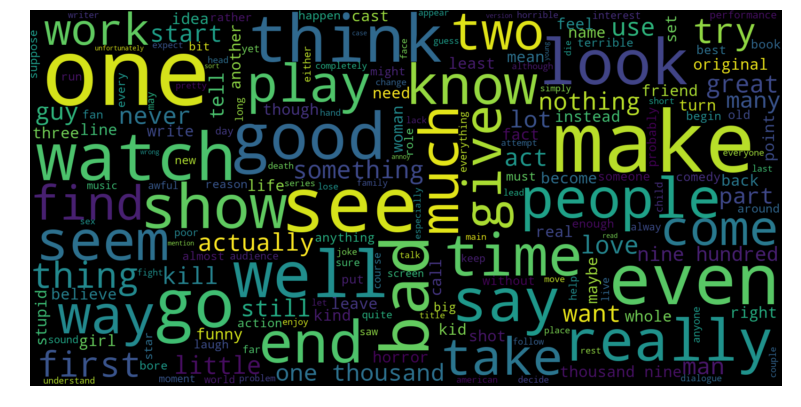
\includegraphics[scale=0.5]{images/wordcloud/negative_wordcloud.png}
  \caption{Les features les plus fréquentes apparaissant dans les avis négatifs du dataset}
  \label{fig:negative_wordcloud}
\end{figure}

\begin{figure}[!ht]
  \centering
  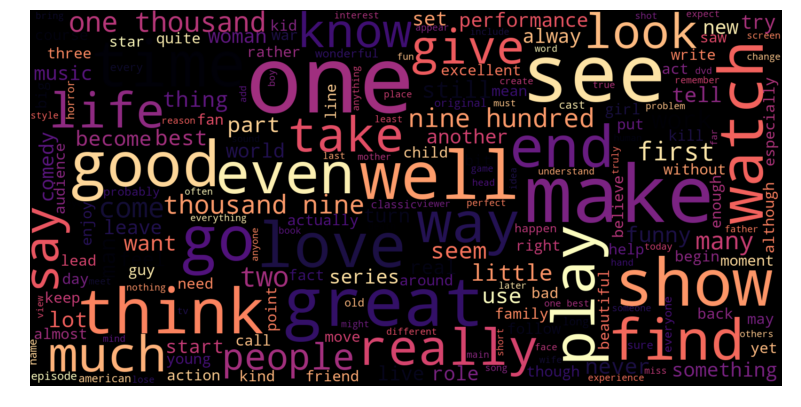
\includegraphics[scale=0.5]{images/wordcloud/positive_wordcloud.png}
  \caption{Les features les plus fréquentes apparaissant dans les avis positifs du dataset}
  \label{fig:positive_wordcloud}
\end{figure}

\section{Traitement de l'ironie}
En s'appuyant sur les visualisations des mots fréquents via les \textbf{Word Clouds}, nous avons remarqué la présence de mots fréquents à polarité négative apparaîssant dans les avis positifs et inversement. Nous avons ainsi conclu que :
\begin{itemize}
  \item soit il y a beaucoup de sarcasme dans les avis ;
  \item soit les avis sont assez longs qu'il faudra analyzer l'ensemble des phrases individuellement et en tirer celles exprimant la polarité globale de l'avis.
\end{itemize}

Malheuresement, faute de temps, nous n'avons pas pu intégrer ces deux techniques à la construction de nos classifieurs et analyser par suite leurs résultats. Vers la fin du projet, nous avons découvert \href{https://github.com/MirunaPislar/Sarcasm-Detection}{l'outil de détection de sarcasme suivant}, sans pouvoir l'intégrer.

\chapter{Conclusion}
L'analyse des sentiments est un domaine en pleine évolution avec diverses applications. Au cours de ces dernières années, il y a eu des progrès monumentales afin de répondre à une forte demande des sociétés cherchant à analyser la qualité de leurs produits et améliorer la fidélité de leurs clients, mais aussi aux besoins des clients recherchant un avis général sur un sujet particulier.

Malgré le fait que nous ayons effectué une vectorisation unigram et bigram, nous avons obtenu de bons résultats. Cependant, cette tâche paraît assez limitée en adoptant une approche machine learning pure, et nécessite des approfondissements en TAL afin d'effectuer plus d'analyses contextuelles et sémantiques améliorant la sélection des features lors de la vectorisation.

Ainsi, dans le but d'améliorer nos résultats, nous pouvons utiliser des techniques contextuelles plus poussées basées sur les POS tags, afin d'identifier l'ironie et le sarcasme. De plus, nous pouvons intégrer une analyse par lexicons utilisant des dictionnaires statiques ou dynamiques permettant de détecter la polarité des avis et rendre notre approche plus hybride.

\begin{appendices}
\chapter{Snapshots des pré-traitements}
\begin{figure}[!ht]
  \centering
  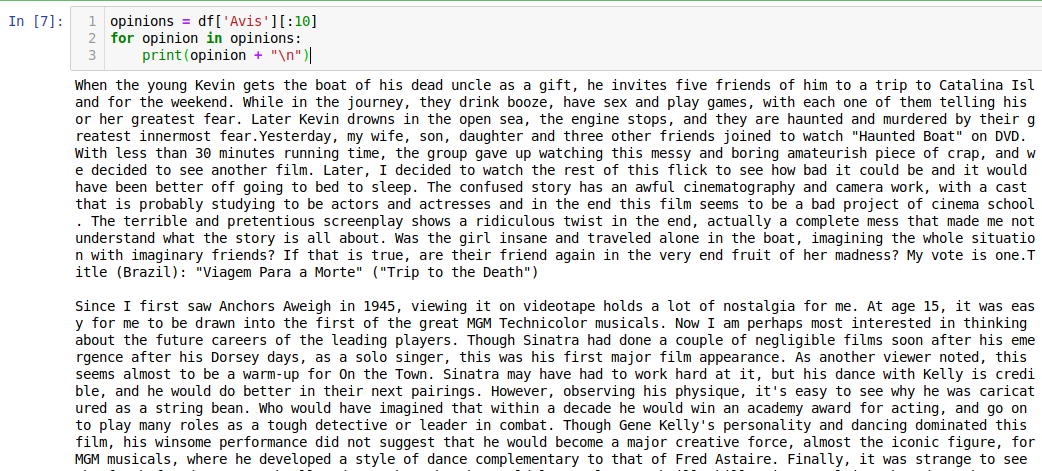
\includegraphics[scale=0.4]{images/snapshots/preprocessing/documents_sample.png}
  \caption{échantillon de documents}
  \label{fig:document_sample}
\end{figure}

\begin{figure}[!ht]
  \centering
  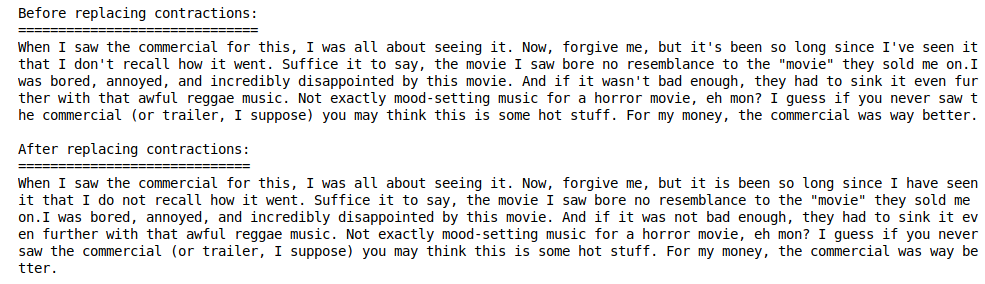
\includegraphics[scale=0.4]{images/snapshots/preprocessing/replace_contractions.png}
  \caption{remplacement des expressions contractées dans un document}
  \label{fig:replace_contractions}
\end{figure}

\begin{figure}[!ht]
  \centering
  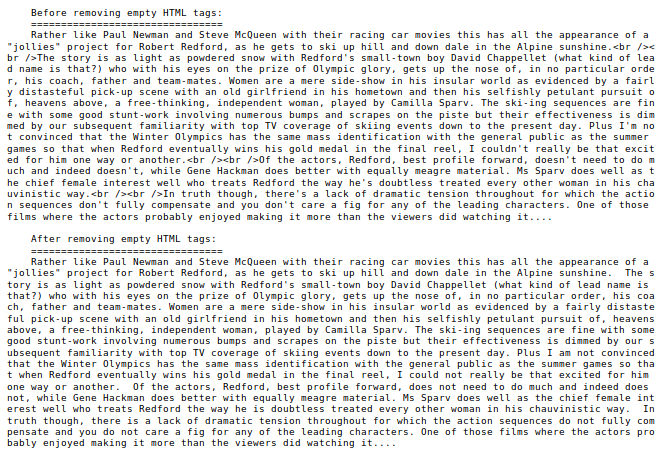
\includegraphics[scale=0.6]{images/snapshots/preprocessing/remove_empty_html_tags.png}
  \caption{suppression des balises auto-fermantes d'un document}
  \label{fig:remove_empty_html_tags}
\end{figure}

\begin{figure}[!ht]
  \centering
  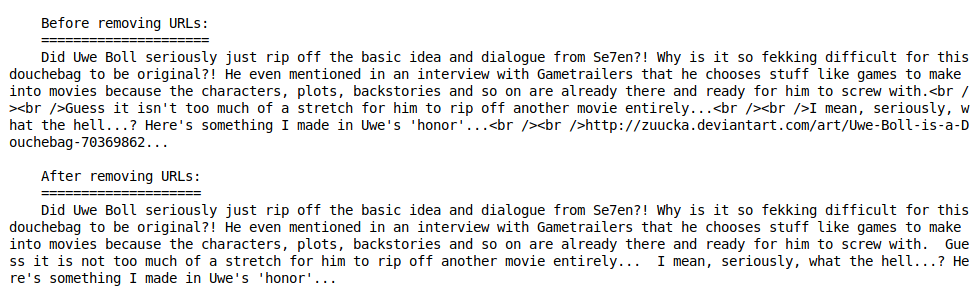
\includegraphics[scale=0.45]{images/snapshots/preprocessing/remove_urls.png}
  \caption{suppression des URLs d'un document}
  \label{fig:remove_urls}
\end{figure}

\begin{figure}[!ht]
  \centering
  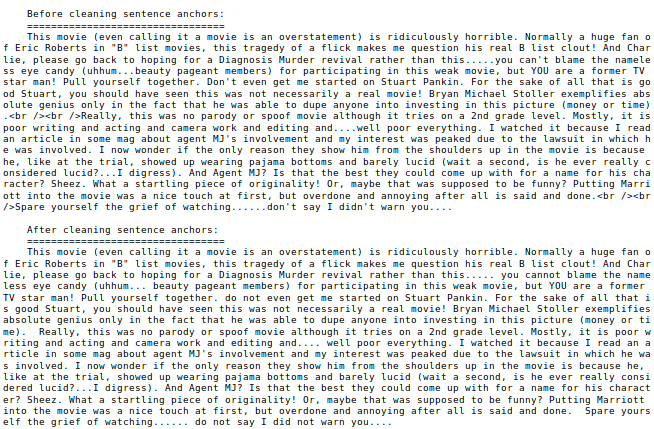
\includegraphics[scale=0.6]{images/snapshots/preprocessing/clean_sentence_anchors.png}
  \caption{nettoyage syntaxique des phrases mal commencées/terminées d'un document}
  \label{fig:clean_sentence_anchors}
\end{figure}

\begin{figure}[!ht]
  \centering
  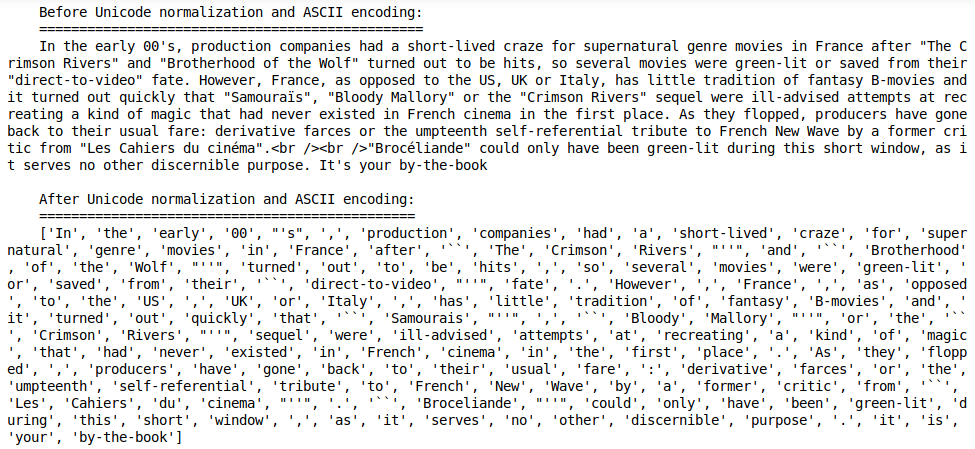
\includegraphics[scale=0.45]{images/snapshots/preprocessing/remove_non_ascii.png}
  \caption{normalisation Unicode, et encodage ASCII des tokens d'un document}
  \label{fig:remove_non_ascii}
\end{figure}

\begin{figure}[!ht]
  \centering
  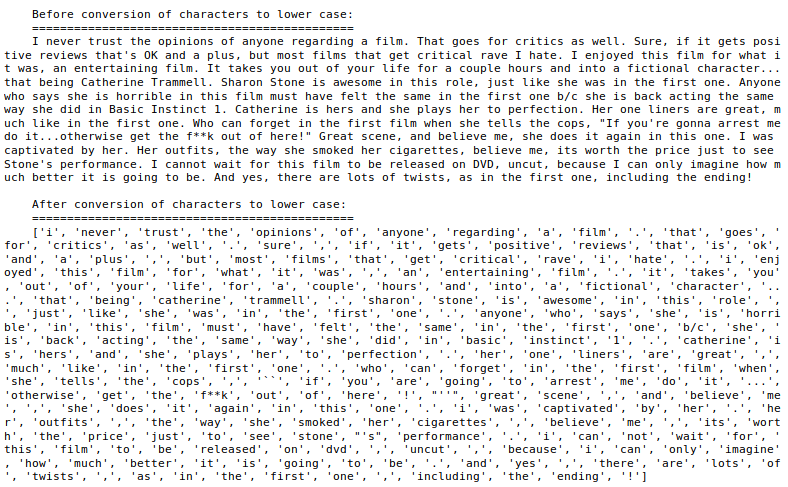
\includegraphics[scale=0.6]{images/snapshots/preprocessing/lowercase.png}
  \caption{conversion en minuscule des tokens d'un document}
  \label{fig:lowercase}
\end{figure}

\begin{figure}[!ht]
  \centering
  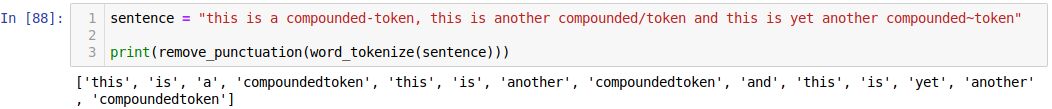
\includegraphics[scale=0.45]{images/snapshots/preprocessing/before_split_characterset.png}
  \caption{suppression des caractères de ponctuation, avant le découpage de tokens composés}
  \label{fig:before_split_characterset}
\end{figure}

\begin{figure}[!ht]
  \centering
  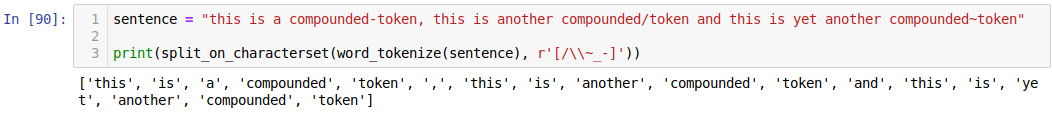
\includegraphics[scale=0.45]{images/snapshots/preprocessing/after_split_characterset.png}
  \caption{découpage des tokens composés}
  \label{fig:after_split_characterset}
\end{figure}

\begin{figure}[!ht]
  \centering
  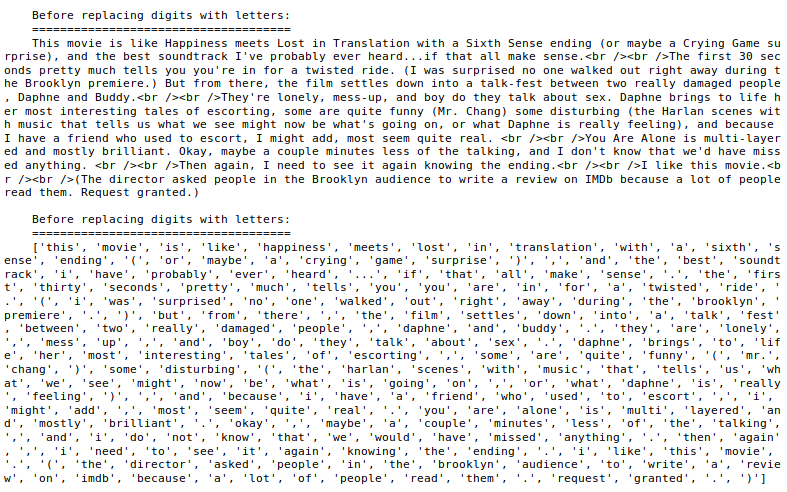
\includegraphics[scale=0.5]{images/snapshots/preprocessing/replace_numbers.png}
  \caption{remplacement des tokens désignant des chiffres par leurs équivalents en lettres}
  \label{fig:replace_numbers}
\end{figure}

\begin{figure}[!ht]
  \centering
  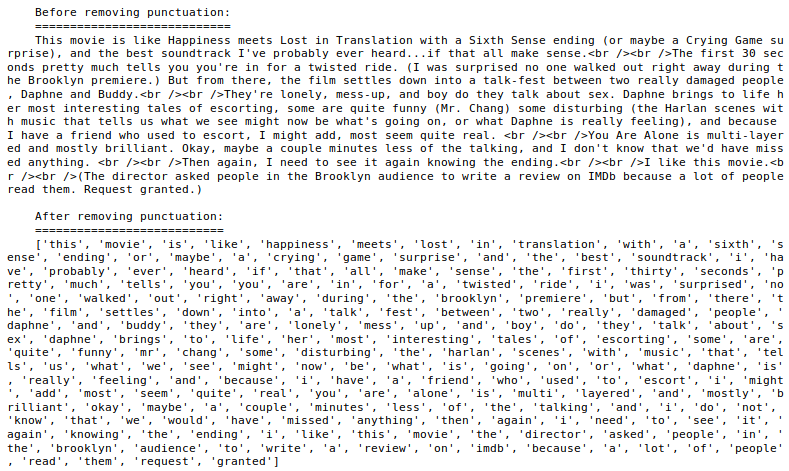
\includegraphics[scale=0.5]{images/snapshots/preprocessing/remove_punctuation.png}
  \caption{suppression des caractères de ponctuation}
  \label{fig:remove_punctuation}
\end{figure}

\begin{figure}[!ht]
  \centering
  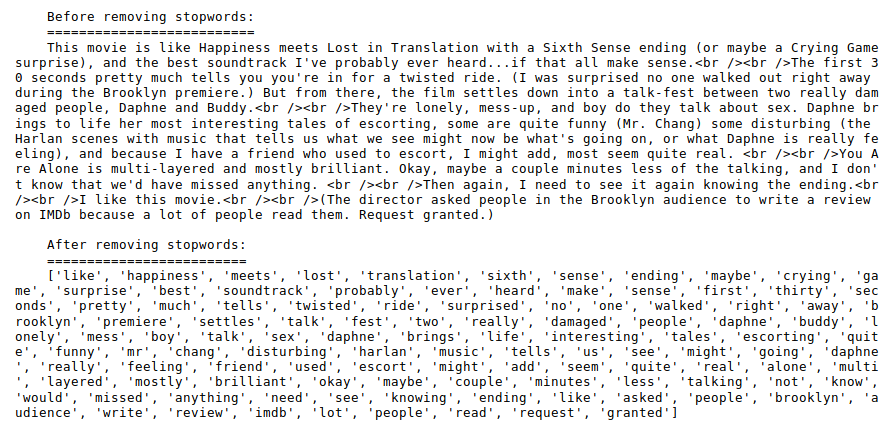
\includegraphics[scale=0.4]{images/snapshots/preprocessing/remove_stopwords.png}
  \caption{suppression des stopwords}
  \label{fig:remove_stopwords}
\end{figure}

\begin{figure}[!ht]
  \centering
  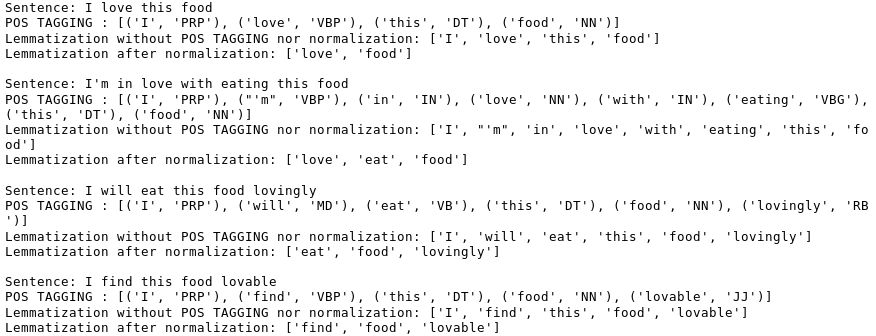
\includegraphics[scale=0.4]{images/snapshots/preprocessing/lemmatization.png}
  \caption{lemmatization en utilisant le POS-Tagging}
  \label{fig:lemmatization}
\end{figure}

\chapter{Snapshots des évaluations des classifieurs}
\begin{figure}[!ht]
  \centering
  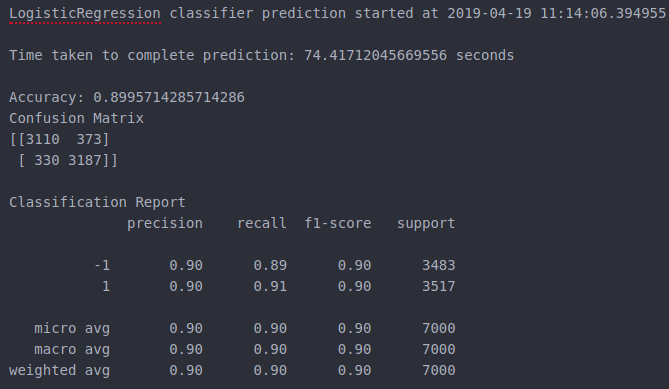
\includegraphics[scale=0.5]{images/snapshots/predictions/logistic_regression/training_set_results.png}
  \caption{Résultats et évaluations de Logistic Regression sur le jeu de test lors de l'apprentissage}
  \label{fig:lr_fit_test}
\end{figure}

\begin{figure}[!ht]
  \centering
  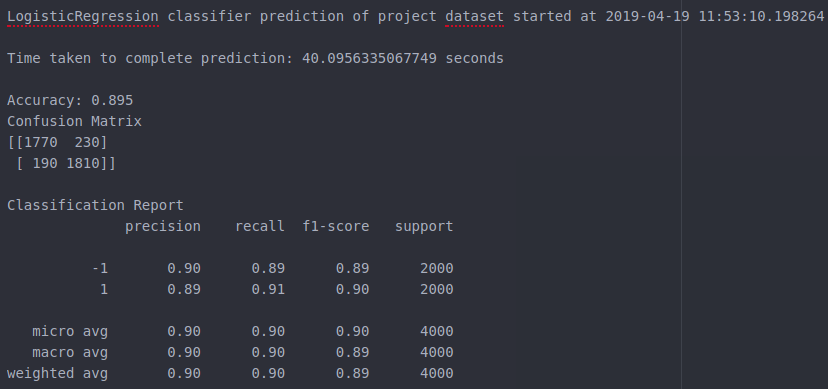
\includegraphics[scale=0.5]{images/snapshots/predictions/logistic_regression/project_dataset_results.png}
  \caption{Résultats et évaluations de Logistic Regression sur le dataset de test du projet}
  \label{fig:lr_project_dataset}
\end{figure}

\begin{figure}[!ht]
  \centering
  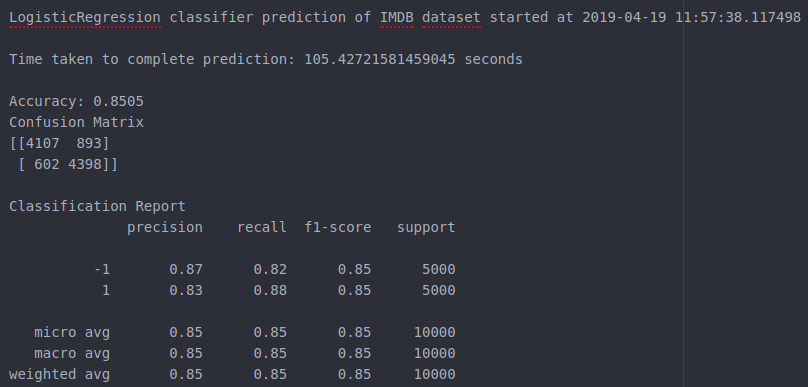
\includegraphics[scale=0.5]{images/snapshots/predictions/logistic_regression/imdb_dataset_results.png}
  \caption{Résultats et évaluations de Logistic Regression sur le dataset IMDB}
  \label{fig:lr_imdb_dataset}
\end{figure}

\begin{figure}[!ht]
  \centering
  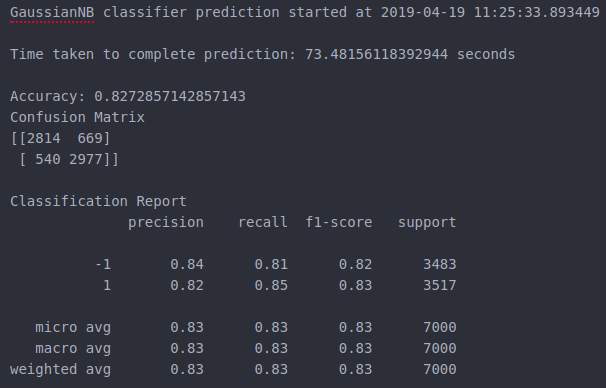
\includegraphics[scale=0.5]{images/snapshots/predictions/gaussian_naive_bayes/training_set_results.png}
  \caption{Résultats et évaluations de Gaussian Naive Bayes sur le jeu de test lors de l'apprentissage}
  \label{fig:gnb_fit_test}
\end{figure}

\begin{figure}[!ht]
  \centering
  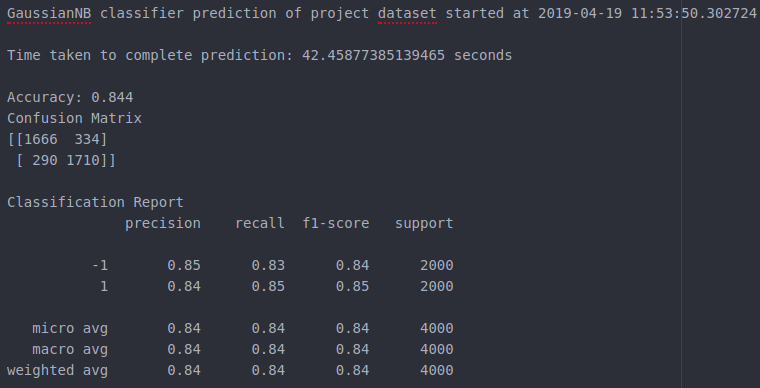
\includegraphics[scale=0.5]{images/snapshots/predictions/gaussian_naive_bayes/project_dataset_results.png}
  \caption{Résultats et évaluations de Gaussian Naive Bayes sur le dataset de test du projet}
  \label{fig:gnb_project_dataset}
\end{figure}

\begin{figure}[!ht]
  \centering
  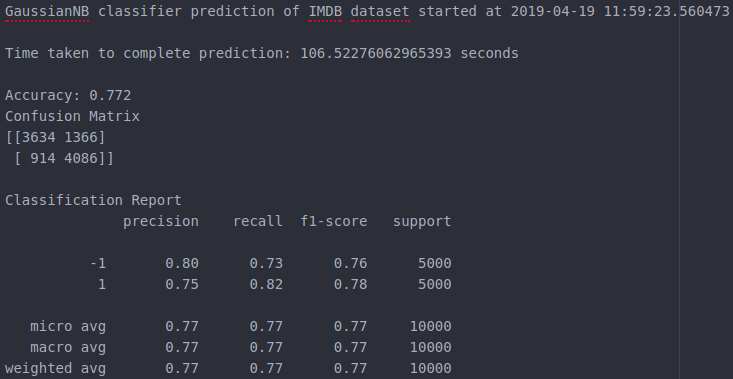
\includegraphics[scale=0.5]{images/snapshots/predictions/gaussian_naive_bayes/imdb_dataset_results.png}
  \caption{Résultats et évaluations de Gaussian Naive Bayes sur le dataset IMDB}
  \label{fig:gnb_imdb_dataset}
\end{figure}

\end{appendices}

\end{document}
